\documentclass[10pt,a4paper]{article}
\usepackage[utf8]{inputenc}
\usepackage{fullpage}
\usepackage{graphicx}
\usepackage{fancyhdr}
\usepackage{occi}
\setlength{\headheight}{13pt}
\pagestyle{fancy}

\newcommand{\doccode}{XXXXX}

% default sans-serif
\renewcommand{\familydefault}{\sfdefault}

% no lines for headers and footers
\renewcommand{\headrulewidth}{0pt}
\renewcommand{\footrulewidth}{0pt}

% header
\fancyhf{}
\lhead{\doccode}
\rhead{\today}

% footer
\lfoot{occi-wg@ogf.org}
\rfoot{\thepage}

% paragraphs need some space...
\setlength{\parindent}{0pt}
\setlength{\parskip}{1ex plus 0.5ex minus 0.2ex}

% some space between header and text...
\headsep 13pt

\setcounter{secnumdepth}{4}

\begin{document}

% header on first page is different
\thispagestyle{empty}

\doccode \hfill Augusto Ciuffoletti, Università di Pisa\\ 
OCCI-WG\\
\rightline {September 22, 2014}\\
\rightline {Updated: \today}

\vspace*{0.5in}

\begin{Large}
\textbf{Open Cloud Computing Interface - Monitoring Extension}
\end{Large}

\vspace*{0.5in}
% My commands!

% This is for signed remarks
%\newcommand{\rem}[2]{\footnote{{\bf Remark by #1}: #2}}
\newcommand{\rem}[2]{}

\newcommand{\oc}[0]{\tt OCCI}
\newcommand{\mi}[0]{{\em mixin}}
\newcommand{\metr}[0]{{\em metric}}
\newcommand{\aggr}[0]{{\em aggregator}}
\newcommand{\publ}[0]{{\em publisher}}
\newcommand{\ent}[0]{{\em Entity}}
\newcommand{\rs}[0]{{\em Resource}}
\renewcommand{\ln}[0]{{\em Link}}
\newcommand{\sens}[0]{{\em Sensor}}
\newcommand{\comp}[0]{{\em Compute}}
\newcommand{\coll}[0]{{\em Collector}}

\underline{Status of this Document}
\input{include/status}

\underline{Copyright Notice}
Copyright \copyright ~Open Grid Forum (2009-2011). All Rights Reserved.

\underline{Trademarks}
OCCI is a trademark of the Open Grid Forum.

\underline{Abstract}
This document, part of a document series produced by the OCCI working
group within the Open Grid Forum (OGF), provides a high-level
definition of a Protocol and API. The document is based upon
previously gathered requirements and focuses on the scope of important
capabilities required to support modern service offerings.


This document {\em defines} an OCCI Extension that provides an API to define the monitoring of Resources defined using the OCCI paradigm. To this end it {\em introduces} two further types: the \sens Resource, that processes metrics, and the \coll Link, that extracts and transports metrics. They are defined as OCCI types whose instances may be refined using OCCI \mi s.

\newpage
\tableofcontents
\newpage

\section{Introduction}

The Open Cloud Computing Interface (OCCI) is a RESTful Protocol and API for all kinds of management tasks. OCCI was originally initiated to create a remote management API for IaaS 1 model-based services, allowing for the development of interoperable tools for common tasks including deployment, autonomic scaling
and monitoring. It has since evolved into a flexible API with a strong focus on interoperability while still offering a high degree of extensibility. The current release of the Open Cloud Computing Interface is suitable to serve many other models in addition to IaaS, including PaaS and SaaS.

In order to be modular and extensible the current OCCI specification is released as a suite of complimentary documents, which together form the complete specification. The documents are divided into three categories consisting of the OCCI Core, the OCCI Renderings and the OCCI Extensions.
\begin{itemize}
\item The OCCI Core specification consists of a single document defining the OCCI Core Model. The OCCI Core Model can be interacted with renderings (including associated behaviours) and expanded through extensions.
\item The OCCI Rendering specifications consist of multiple documents each describing a particular rendering of the OCCI Core Model. Multiple renderings can interact with the same instance of the OCCI Core Model and will automatically support any additions to the model which follow the extension rules defined in OCCI Core.
\item The OCCI Extension specifications consist of multiple documents each describing a particular extension of the OCCI Core Model. The extension documents describe additions to the OCCI Core Model defined within the OCCI specification suite. They do not require changes to the HTTP Rendering specifications as of this version of the specification.
\end{itemize}

This document describes an {\em OCCI Extension} useful to define a monitoring infrastructure. Its applicability extends to fault detection, billing, and to the implementation of a verifiable server level agreement.

The API should be sufficiently expressive to allow the user to arrange a monitoring infrastructure in the way that best suits his needs: notably, the existence of an agreed interface enables the user to manage distinct cloud providers, possibly at the same time, in a uniform way.

The importance of a configurable monitoring infrastructure emerges in many scenarios, starting from the simple case of the user that wants to monitor the activity of an array of servers, to composite use cases, where the user is in fact an intermediate service provider, that provides services to third party users in a multi-provider environment (see figure \ref{img:scenario}): in that case, the intermediate provider may decide to offer quality of service options that differ from that of the low level provider, thus needing to perform specific measurements on the infrastructure leased by the low level provider(s). The tools provided by an API that describes a monitoring infrastructure must be flexible enough to meet all degrees of complexity.

\begin{figure}[b]
\centering
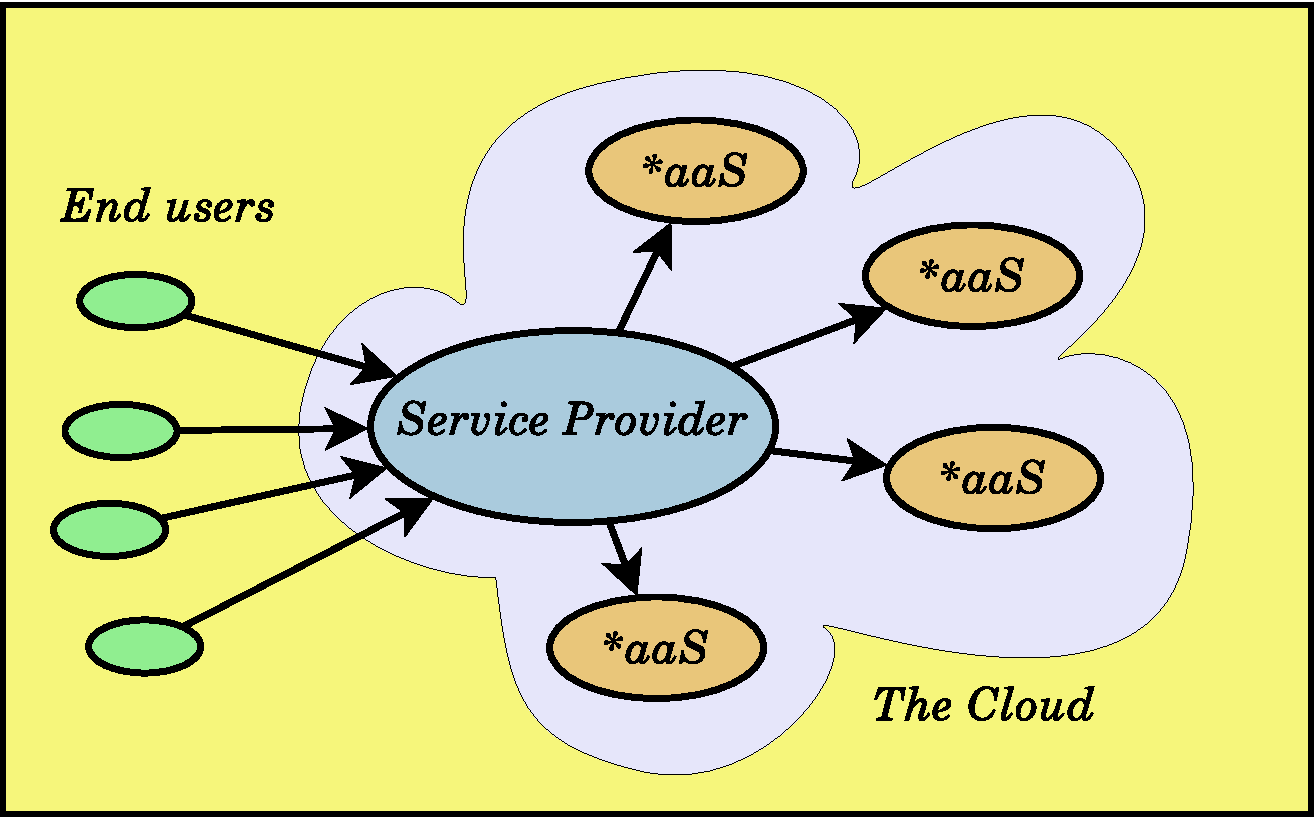
\includegraphics[width=0.5\textwidth]{figs/multilayer.pdf}
\caption{A multilayer and multiprovider scenario \label{img:scenario}}
\end{figure}

The communication of measurements inside and outside the monitoring infrastructure is another issue the framework must be flexible about. In fact, the amount of information that is produced by a measurement activity may range from negligible to ``big data'' dimensions, with various degrees of confidentiality. Also in this respect the API should be sufficiently expressive to allow the user to describe the task, but leaving the provider the options to find a solution fitting the scale of the problem.

One relevant fact about monitoring infrastructures is that it is extremely difficult to give a {\em detailed} framework for them that extends its validity to any conceivable use case or provider. The reason is that each of them exhibits local variants that do not fit a rigid approach. Also, the metrics that are used to evaluate the performance of the system are many, and subject to continuous changes due to the introduction of new technologies. Thus we have made an effort to introduce a generic schema that can be adapted so to effectively describe the relevant aspects of a monitoring infrastructure, but that does not interfere with details that can be transparently dealt with by the provider, and the OCCI Core Model \cite{occi:core} is well suited for the task. Furthermore, we claim that the specifications given in this document can find an application in environments other than computing infrastructures, since we abstract from the details that characterize cloud infrastructure resources.

The approach followed in this document is similar to that found in the infrastructure document (GFD-P-R.184 \cite{occi:infrastructure}): the monitoring capability is described as an {\em OCCI-Link}, the {\em Collector}. The {\em source} of a \coll\ is the monitored resource that originates measurements that are delivered to the {\em target} resource. With the creation of a \coll\ instance the user indicates a specific monitoring technique applied on the {\em source}. The processing of the measurements and their delivery are described by an {\em OCCI-Resource}, the {\em Sensor}. With the creation of a \sens\ instance the user describes how metrics are collected from a \coll\ and how they are made available: for instance a \sens\ might produce the average load of an array of servers and publish it on a web page.

The three aspects of monitoring that we have thus outlined -- namely measurement, processing, and publishing -- may be further specified through the association of specific \mi s to a \sens\ or \coll\ instance: this leaves the specific provider free to provide an opaque solution, or to allow the user to customize one.

%The simplest case of a monitoring infrastructure consists of a single \coll\ that links a monitored resource to a \sens\ that publishes the raw metrics; it is illustrated in figure \ref{fig:onestage}.

%\begin{figure}
%\centering
%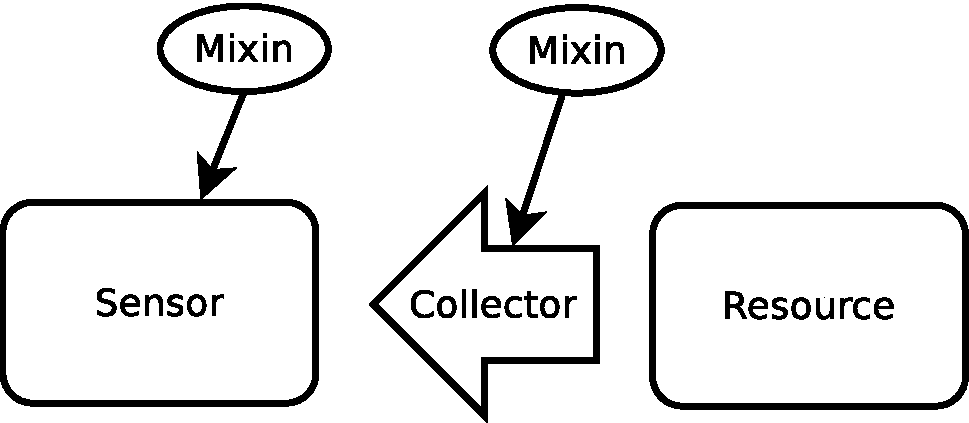
\includegraphics[width=0.5 \linewidth]{onestage.pdf}
%\caption{The simplest case: one \coll\ and one \sens\ \label{fig:onestage}}
%\end{figure}

The OCCI-Monitoring API is designed to scale from very simple use cases, that the user can define with minimal effort, to complex cases, like multilayer monitoring infrastructures. The same basic building blocks are used at any degree of complexity.

%The {\em Resource Management} box stands for a resource that is the end-user of the monitoring activity. It's {\em Kind} is bound to the publishing technique used in the \coll . It may be, for instance, a {\em Compute} resource that embeds a load balancing or accounting functionality, or a yet to define {\em Mailbox} resource where periodic reports are posted. 

\rem{author}{Why not a mixin to the monitored resource directly? I envision problems emerging with the implementation. A resource can be ``prepared'' for monitoring, but the way in which the Monitoring Link will interact with such preparation is not clear. In addition, consider that the same tool might be the target of several links, with distinct configuration parameter. How can the control parameters of the mixin be exposed in such a case? Instead, if the mixin is embedded in the link, it is the responsibility of the link implementation to configure it, and to couple it with the publishing technology indicated in the link}

This document considers the monitoring activity as a real-time activity. Using the OCCI-Monitoring API the user defines the frequency with which measurements are collected, as well as the time lapse during which the measurement takes place. This excludes from the range of applicability of this document those cases that envision the event driven notification of a state change: the OCCI-notification extension \ref{occi-notification} covers this case.

Summarizing, the specifications introduced in this document require that the conformant provider implements two {\em Kind}s: the {\em \coll } and the {\em \sens }. Three well-known tagging \mi s are also defined to enable the classification of \mi s that are specific for the provider: namely {\em Metric} to specify the production of measurement, {\em Aggregator} for their processing, and {\em Publisher} for their publication. Such tags are used to identify and apply restrictions to provider-specific \mi s, for the sake of interoperability.

\begin{figure}
\centering
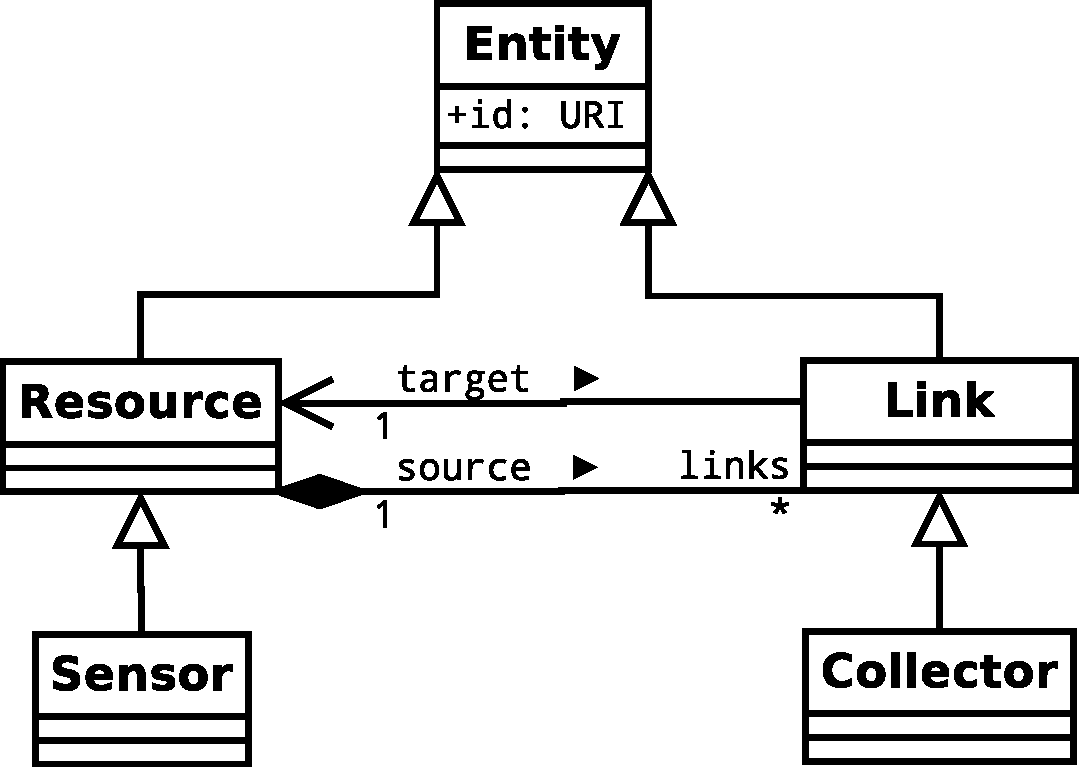
\includegraphics[width=0.3\textwidth]{figs/Monitoring_UML.pdf}
\caption{Class inheritance diagram for OCCI-monitoring}
\end{figure}

\section{Specification of the compliant server}

The compliant server MUST implement the {\em kind}s in table \ref{tab:kinds}, and the {\em mixin}s in table \ref{tab:mixin}.

\mytablefloat{
        \label{tab:kinds}The immutable model attributes of the \sens\ and of the \coll\ kinds.
        The base URL {\bf http://schemas.ogf.org/occi} has been replaced with
        {\bf $<$schema$>$} in this table for a better readability experience. 
        } {
        \begin{tabular}{llllll}
        \toprule
        Term & Scheme & Title & Attributes & Actions & Parent\\
        \colrule
        sensor &  $<$schema$>$/monitoring\# & Sensor Resource
        & see Table \ref{tab:sensor} & \{\} &  $<$schema$>$/core\#resource\\
        collector &  $<$schema$>$/monitoring\# & Collector Link
        & see Table \ref{tab:collector} & \{\} & $<$schema$>$/core\#link \\
        \botrule
        \end{tabular}
}

The attributes of the two kinds are illustrated in section \ref{sec:sensor} and in section \ref{sec:collector} respectively.

The mixins have no capabilities: they are used as tags for other mixins with given features, as described in section \ref{sec:metric}, \ref{sec:aggregator}, \ref{sec:publisher}.


\mytablefloat{
        \label{tab:mixin}The immutable model attributes of the {\em Metric}, {\em Aggregator} and {\em Publisher} mixins.
        The base URL {\bf http://schemas.ogf.org/occi} has been replaced with
        {\bf $<$schema$>$} in this table for a better reading experience. 
        } {
        \begin{tabular}{lllllll}
        \toprule
        Term & Scheme & Title & Attributes & Actions & Depends & Applies \\
        \colrule
        metric &  $<$schema$>$/monitoring\# & Metric Mixin 
        & \{\} & \{\} & \{\} & $<$schema$>$/monitoring\#collector \\
        aggregator &  $<$schema$>$/monitoring\# & Aggregator Mixin 
        & \{\} & \{\} & \{\} & $<$schema$>$/monitoring\#sensor \\
        publisher &  $<$schema$>$/monitoring\# & Publisher Mixin 
        & \{\} & \{\} & \{\} & $<$schema$>$/monitoring\#sensor \\
        \botrule
        \end{tabular}
}
\subsection{The \sens\ resource \label{sec:sensor}}

\mytablefloat{
        \label{tab:sensor} 
        \hl{Attribute}s of the Sensor resource.
}{
\begin{tabular}{lp{1.5cm}p{1cm}lp{5.5cm}}
\toprule
Attribute&Type&Multi\-plicity&Mutability&Description\\
\colrule
occi.sensor.timebase & string & 0..1 & true & Base time reference (ISO8601) \\  
occi.sensor.timestart &	number & 0..1 & true & Start time offset (seconds) \\
occi.sensor.timestop & number	& 0..1 & true & Stop time offset (seconds) \\
occi.sensor.period & number & 1 & true & Time between two following measurements (seconds) \\
occi.sensor.granularity & number & 0..1 & true & Granularity of time measument (seconds) \\
occi.sensor.accuracy & number & 0..1 & true & Accuracy of time measument (seconds) \\
\botrule
\end{tabular}
}

The {\em kind} instance assigned to the \sens\ type is {\tt http://schemas.ogf.org/occi/monitoring\#sensor}, as in table \ref{tab:kinds}. The attributes of the \sens\ (see table \ref{tab:sensor}) describe the real-time properties of the sequence of metric values: the time interval during which the monitoring activity is in effect, and its frequency.

The start of the monitoring activity is determined as the sum between a reference date and time ({\tt timebase}) and an offset ({\tt timestart}). Another offset determines the time when the monitoring activity terminates ({\tt timestop}). The attributes may be left undefined, to indicate that the monitoring activity persists for the lifetime of the sensor. A negative {\tt timebase} indicates that the monitoring activity is suspended. The three attributes can be modified by the user to dynamically control the monitoring activity.

The frequency of the monitoring operation is controlled by a value that corresponds to the time lapse between successive samples ({\tt period}). This attribute is required.

The precision of the time scale is defined by two attributes, the {\tt granularity} and the {\tt accuracy}. The former represents the minimum distance in time between two following time values, the latter indicates the maximum distance between the measured time and the real time. These attributes may be left unspecified.

The server SHOULD respond with an error, without allocating the \sens\ resource, when the period of operation is partially in the past, or when the stop time precedes the start time. The server SHOULD NOT respond with an error when the {\tt period}, the {\tt granularity} or the {\tt accuracy} cannot be met. Instead, it SHOULD attempt a {\em best fit} of the requested values, setting the appropriate values for the attributes. The server SHOULD fill undefined {\tt granularity} or the {\tt accuracy} attributes with worst case values. 

\subsection{The \coll\ link \label{sec:collector}}

\mytablefloat{
        \label{tab:collector}%
        \hl{Attribute}s of the Collector link.
}{
\begin{tabular}{lp{1.5cm}p{1cm}lp{5.5cm}}
\toprule
Attribute&Type&Multi\-plicity&Mutability&Description\\
\colrule
occi.collector.period & number & 1 & true & Time between two following measurements (seconds) \\
occi.collector.granularity & number & 0..1 & true & Granularity of time measument (seconds) \\
occi.collector.accuracy & number & 0..1 & true & Accuracy of time measument (second\\
\botrule
\end{tabular}
}

The {\em kind} instance assigned to the \coll\ type is {\tt http://schemas.ogf.org/occi/monitoring\#collector}, as in table \ref{tab:kinds}. The attributes of the \coll\ (see table \ref{tab:collector}) model the activity that extracts measurements from a destination {\em resource} and the transfer of such measurements to a source \sens. The {\em source} of a \coll\ MUST be a \sens.

The OCCI attributes of the \coll\ define the timing of the monitoring activity.
The execution rate is defined using three attributes: the rate itself (\verb|period|), and the quality of the timing ({\tt granularity} and {\tt timing}). All three values can be left unspecified.

The server SHOULD NOT respond with an error when the {\tt period}, the {\tt granularity} or the {\tt accuracy} cannot be met. Instead, it SHOULD attempt a {\em best fit} of the requested values, setting the appropriate values for the attributes. The server SHOULD fill undefined {\tt granularity} or the {\tt accuracy} attributes with worst case values. 

\subsection{Features of the \mi s that depend on the {\em Metric} tag \label{sec:metric}}

The {\em mixin} instance assigned to the {\em metric} mixin is {\tt http://schemas.ogf.org/occi/monitoring\#metric}, as in table \ref{tab:mixin}. The {\em metric} mixin has no capabilities, and is used as a tag for mixins that customize a \coll\ link, by specifing the collected metrics and the measurement process.

The OCCI attributes of a {\em mixin} that depends on the {\em metric} tag are divided into two groups:
\begin{itemize}

\item Metric attributes: they represent the delivered measurements. They are a {\em String} identifier that is associated with an {\em output channel} (see section \ref{sec:channel});
\item Control attributes: they control the operation of the measurement activity.
\end{itemize}

\subsection{Features of the \mi s that depend on the {\em Aggregator} tag \label{sec:aggregator}}

The {\em mixin} instance assigned to the {\em aggregator} mixin is {\tt http://schemas.ogf.org/occi/monitoring\#aggregator}, as in table \ref{tab:mixin}. The {\em aggregator} mixin has no capabilities, and is used as a tag for mixins that customize a \sens\ resource, by specifing how raw metrics are processed before being published.

The OCCI attributes of a \mi\ that depends on the {\em aggregator} tag are divided into three groups:

\begin{itemize}

\item Input attributes: they bind an input of the aggregating algorithm with the metrics coming from monitored resources connected with outgoing \coll s. They are {\em String} identifiers that are associated with an {\em input channel} (see section \ref{sec:channel}).
\item Control attributes: they control the operation of the aggregating function;
\item Metric attributes: they represent the delivered measurements. They are a {\em String} identifier that is associated with an {\em output channel} (see section \ref{sec:channel}).
\end{itemize}

\subsection{Features of the \mi s that depend on the {\em Publisher} tag \label{sec:publisher}}

The {\em mixin} instance assigned to the {\em publisher} mixin is {\tt http://schemas.ogf.org/occi/monitoring\#publisher}, as in table \ref{tab:mixin}. The {\em publisher} mixin has no capabilities, and is used as a tag for mixins that customize a \sens\ resource, by specifing how metrics are published.

The OCCI attributes of a \mi\ that depends on the {\em publisher} tag are divided into two groups:

\begin{itemize}
\item Input attributes: they bind the publishing process with the metrics produced by metric or aggregator mixins. They are {\em String} identifiers that are associated with an {\em input channel} (see section \ref{sec:channel}).;
\item Control attributes: they control the process used to publish input attributes.
\end{itemize}

\subsection{The scope and the monitoring pipe \label{sec:channel}}

The three types of mixins --- namely, {\em metric}, {\em aggregator}, and {\em publisher} --- are meant to represent the three stages of a pipe. Measurements flow across the three stages, from the monitored resource to the point where they are published. The available plugins are the tools the user has to define and customize his monitoring infrastructure.

In case the provider offers the user basic building blocks, instead of pre-configured monitoring schemas, the API must be powerful enough to define the flow of data between such building blocks. Input and output attributes allow this: when such attributes share the same value (or {\em channel} identifier) measuments flow from input ones to output ones.

The visibility of {\em channel} identifiers is limited within a \sens\ and its outgoing \coll. For this reason all of them are collectively indicated as the {\em scope} of that \sens .

According with the core properties of resources and links (see \cite{occi:core}), the removal of a \sens\ determines the removal of all \coll s in its scope.

\section{Conformance profiles}

The definition of conformance profiles is appropriate because the provision of an interface for the management of a monitoring infrastructure is optional. 

\begin{description}

\item[Profile 0] The \coll\ and \sens\ {\em Kind} s MUST NOT be implemented: attempt of instantiating such {\em Kinds} fails.  In an HTTP rendering a POST and GET over the corresponding URI returns {\tt 404 Notfound}. The {\em Aggregator}, {\em Metric}, and {\em Publisher} \mi s MUST NOT be implemented: discovery fails. In an HTTP rendering a GET over the \mi\ returns {\tt 404 Notfound}; 

\item[Profile 1] The \coll\ and \sens\ {\em Kind} s MUST be implemented, and the user MUST be allowed to create new instances of such {\em Kinds}.  In an HTTP rendering a POST or a GET over the corresponding URI return respectively {\tt 201} and {\tt 200}. In case of error, the server MUST NOT return {\tt 404 Notfound}. The {\em Aggregator}, {\em Metric}, and {\em Publisher} \mi\ MUST be implemented, and discovery is successful. The server MUST NOT allow to introduce {\em depends} relationships with the {\em Aggregator}, {\em Metric}, and {\em Publisher} \mi s. In an HTTP rendering, a POST over their URIs returns {\tt 405 Method Not allowed}; 

\item[Profile 2]  The \coll\ and \sens\ {\em Kind} s MUST be implemented, and the user MUST be allowed to create new instances of such {\em Kinds}.  In an HTTP rendering a POST and GET over the corresponding URI returns respectively {\tt 201} and {\tt 200}. In case of error, the server MUST NOT return {\tt 404 Notfound}. The \aggr , \metr , and \publ\ \mi s MUST be implemented, and discovery is successful. The user MUST be allowed to introduce {\em depends} relationships with the  \aggr , \metr , and \publ\ \mi s. In an HTTP rendering, a POST over their URIs returns {\tt 200}.

\end{description}

\rem{
\section{Related works}

The topic of Cloud Service Level Agreement has been extensively studied in a number of research projects, and there are results that have an impact on Cloud Monitoring: a report \cite{EU-SLA} of the European Union illustrates the results in the field. We have taken input from this activity in the design of this API.

In particular, we considered the need of taking into account the presence of {\em composite services} encompassing several providers for their implementation. Tightly related ot this is the need of representing multilevel monitoring infrastructures, a fact anticipated by the results of the SLA@SOI EU project. The results of the {\em Stream} project highlight how monitoring data may introduce {\em big data} issues, that need specific, flexible solutions on the provider's side: this is one of the reasons that induced the introduction of opaque {\em connectors} that hide sophisticated, rapidly evolving technologies. The IRMOS project puts an accent on timing requirements for multimedia services, that justify the attention we paid to define and qualify timing attributes. Many project made precise statements about the specific metrics that describe the Service Level for specific types of resource: the mPlane project addresses specifically the metrics for Network resources, while Cloud4SOA focusses on the relevance of an agreed set of standard metrics.

In the design of this API we also took advantage of the experience gained during the CoreGRID EU-project \cite{cur:08:a}, where we implemented a Grid monitoring infrastructure, in its turn inspired by many previous works (see the bibliography in the paper).

The reading of the CompatibleOne prototype \cite{mar12a} is an Open Source project aimed at developing an OCCI-compliant Cloud Infrastructure: its interface, that already covers monitoring and SLA aspects, helped with a concrete view of a possibile interface. It has been enlightening concerning (among the rest) the need and possibility of modularizing the monitoring part.

The 2012 revision of the OCCI core model \cite{occi:core} has been used as a reference.

}

\section{Security issues}
The OCCI Notification specification is an extension to the OCCI Core
and Model specification \cite{occi:core}; thus the same security
considerations as for the OCCI Core and Model specification apply
here.

\rem{\label{s:security}

The API described in this document relies on the same mechanism as the basic OCCI API, of which it is an extension. In its turn, the OCCI API is designed according with a RESTFul model, a style of exposing a web service to the users.

The way this API is exposed inherits the security aspects of the RESTFul model, that can be summarized as follows:

\begin{itemize}
\item the web site MUST be protected to allow access only to authorized users, and to protect the content of the communication;
\item the content uploaded on the web site by the user (using POST) MUST be protected;
\item the content cached on third party sites not directly accessible by the user and by the provider (proxies etc.) MUST be protected.
\end{itemize}

We stress that these security warnings are shared with any ReStFul API.

The provider must ensure that a user defined \mi\ does not compromise the security of other services. The provider may attain this by restricting the functionalities associated to a \mi\ (the limit case is the provision of templates) or run the functionalities associated to a \mi\ in a protected environment (e.g., as a Unix user in a chroot jail). This issue is shared with the OCCI model.

Concerning the kind of monitoring infrastructure deployed using the \sens\ and the \coll , security aspects are managed using appropriate \mi s. For instance the \coll\ might be associated with a \mi\ describing a secure transport protocol, while the sensor might be configured to be accessible only from authenticated users (?). The provider SHOULD offer the user a set of predefined \mi s that introduce the appropriate level of security. User defined \mi s SHOULD be avoided for this kind of options.
}

\section{Glossary}
\label{sec:glossary}
\todo{update glossary}

\begin{tabular}{l|p{12cm}}
Term & Description \\
\hline
\hl{Action} & An OCCI base type. Represents an invocable operation on a \hl{Entity} sub-type instance or collection thereof. \\

\hl{Attribute} & A type in the OCCI Core Model. Describes the name and properties of attributes found in \hl{Entity} types. \\

\hl{Category} & A type in the OCCI Core Model and the basis of the OCCI type identification mechanism. The parent type of \hl{Kind}. \\

capabilities & In the context of \hl{Entity} sub-types {\bf  capabilities} refer
  to the OCCI \hl{Attribute}s and OCCI \hl{Action}s exposed by an {\bf entity
  instance}. \\

\hl{Client} & An OCCI client.\\

\hl{Collection} & A set of \hl{Entity} sub-type instances all associated to a particular \hl{Kind} or \hl{Mixin} instance. \\

\hl{Entity} & An OCCI base type. The parent type of \hl{Resource} and \hl{Link}. \\

entity instance & An instance of a sub-type of \hl{Entity} but not an instance
  of the \hl{Entity} type itself.  The OCCI model defines two sub-types of
  \hl{Entity}, the \hl{Resource} type and the \hl{Link} type.  However, the
  term {\em entity instance} is defined to include any instance of a
  sub-type of \hl{Resource} or \hl{Link} as well. \\

\hl{Kind} & A type in the OCCI Core Model. A core component of the OCCI classification system. \\

\hl{Link} & An OCCI base type. A \hl{Link} instance associates one \hl{Resource} instance with another. \\

\hl{Mixin} & A type in the OCCI Core Model. A core component of the OCCI classification system. \\

mix-in & An instance of the \hl{Mixin} type associated with an {\em entity
 instance}. The ``mix-in'' concept as used by OCCI {\em only} applies to
 instances, never to \hl{Entity} types. \\

model attribute & An internal attribute of a the Core Model which is {\em not}
  client discoverable. \\

\hl{OCCI} & Open Cloud Computing Interface. \\

OCCI base type & One of \hl{Entity}, \hl{Resource}, \hl{Link} or \hl{Action}. \\

OCCI Action & see \hl{Action}. \\
OCCI Attribute & A client discoverable attribute identified by an instance of the \hl{Attribute} type. Examples are \hl{occi.core.title} and \hl{occi.core.summary}. \\
OCCI Category & see \hl{Category}. \\
OCCI Entity & see \hl{Entity}. \\
OCCI Kind & see \hl{Kind}. \\
OCCI Link & see \hl{Link}. \\
OCCI Mixin & see \hl{Mixin}. \\

OGF & Open Grid Forum. \\

\hl{Resource} & An OCCI base type. The parent type for all domain-specific \hl{Resource} sub-types. \\

resource instance & See {\em entity instance}. This term is considered obsolete. \\

tag & A \hl{Mixin} instance with no attributes or actions defined. \\

template & A \hl{Mixin} instance which if associated at instance
creation-time pre-populate certain attributes. \\

type & One of the types defined by the OCCI Core Model.  The Core Model types are
 \hl{Category}, \hl{Attribute},
 \hl{Kind}, \hl{Mixin}, \hl{Action}, \hl{Entity}, \hl{Resource}
 and \hl{Link}. \\

concrete type/sub-type & A concrete type/sub-type is a type that can be instantiated.\\

URI & Uniform Resource Identifier. \\
URL & Uniform Resource Locator. \\
URN & Uniform Resource Name. \\
\end{tabular}

 
\section{Contributors}

\textbf{Augusto Ciuffoletti (corresponding author)} \\
Dept. of Computer Science \\
L.go B. Pontecorvo - Pisa\\
Italy \\
Email: augusto.ciuffoletti@gmail.com \\

\textbf{Andrew Edmonds}\\
Institute of Information Technology \\
Zürich University of Applied Sciences \\
Zürich \\
Switzerland \\
Email: andrew.edmonds@zhaw.ch

\textbf{Metsch, Thijs} \\
Intel Ireland Limited \\
Collinstown Industrial Park \\
Leixlip, County Kildare, Ireland
Email: thijsx.metsch@intel.com

\textbf{Ralf Nyren} \\
Email: ralf@nyren.net 


\section{Intellectual Property Statement}
\input{include/ip}

\section{Disclaimer}
This document and the information contained herein is provided on an
``As Is'' basis and the OGF disclaims all warranties, express or
implied, including but not limited to any warranty that the use of the
information herein will not infringe any rights or any implied
warranties of merchantability or fitness for a particular purpose.


\section{Full Copyright Notice}
Copyright \copyright ~Open Grid Forum (2009-2016). All Rights Reserved.

This document and translations of it may be copied and furnished to
others, and derivative works that comment on or otherwise explain it
or assist in its implementation may be prepared, copied, published and 
distributed, in whole or in part, without restriction of any kind,
provided that the above copyright notice and this paragraph are
included as references to the derived portions on all such copies
and derivative works. The published OGF document from which such works
are derived, however, may not be modified in any way, such as by removing
the copyright notice or references to the OGF or other organizations,
except as needed for the purpose of developing new or updated OGF documents
in conformance with the procedures defined in the OGF Document Process,
or as required to translate it into languages other than English. OGF,
with the approval of its board, may remove this restriction for inclusion
of OGF document content for the purpose of producing standards in cooperation
with other international standards bodies. 

The limited permissions granted above are perpetual and will not be
revoked by the OGF or its successors or assignees.




%\section{Acknowledgments}

%Include if desired. Contributors to the document may also be listed in the previous section.

\bibliographystyle{IEEEtran}
\bibliography{references}

\end{document}
\appendix

\section*{Appendix - Examples: from simple to complex}

The OCCI Monitoring API is able to meet the demands of a wide range of users. It is understood that an application that has a limited interest in monitoring (for instance to trigger human intervention to cope with a fault) wants an interface able to configure in a straightforward way a simple strategy. In contrast, the user that is faced with a complex infrastructure and tight quality requirements needs an expressive interface. On the provider side as well there is interest for the possibility of restricting the monitoring tools available to certain users to a restricted set, with limited capabilities. The challenge for the overall scheme is to cover the whole range, from simple to complex.

In this appendix we explore use cases starting from a very simple one, approached in a simplistic way. The involved {\em Entities} are described by listing their attributes; both model attributes, in bold, and OCCI attributes. We recall that model attributes are not discoverable by the client, while OCCI attributes are.

\subsection*{Case 1: too simple}

We start from an extremely simple case, that the user wants to implement trading off efficiency for simplicity. We focus on the {\tt iostat} \mi\ used above, that a user wants to use to be warned about the overload of a server {\tt \small vm1}.

The simplistic, yet suboptimal, solution is to associate the server with the monitoring tool. At a certain point in time, when the cpuutilization is $78\%$, the state of a certain server might be the following:

{
\small
\begin{tabular}{l|l}
Attribute                         & value \\ \hline
{\bf id}                          & urn:acme:user529/vm1 \\
{\bf kind}                        & compute \\
{\bf mixin}                       & iostat-here \\
occi.compute.architecture         & x86   \\
occi.compute.cores                & 4     \\ 
occi.compute.hostname             & vm1   \\            
occi.compute.speed                & 3     \\                  
occi.compute.memory               & 250   \\
com.acme.iostat.cpuutilization    & 78    \\                     
com.acme.iostat.what              & user  \\
\end{tabular}
}

The provider declares to update the {\em metric} attribute {\tt \small cpuutilization} every 10 minutes, and the user is happy with that latency. From time to time the user will download the REST resource associated with the {\em Compute Resource} and parse out the value of the attribute, that will be processed in user's premises.

Let's consider a possible implementation on provider's side. Whenever the user associates the {\tt \small iostat} mixin to the {\em Compute Resource}, the Cloud Management Infrastructure will install and launch a script that performs the call to the {\tt \small iostat} command, and then sends the data to the Cloud Management Interface. In its turn, the Cloud Management server will update the record describing the Compute Resource. At this time any cached content of the same record should become invalid.

It is a quite complex operation that hardly fits in a REST environment.

This solution, which is admissible for our API, is extremely simple for the user, but extremely inefficient and complex for the provider. Let us explore an slightly more complex alternative that exhibits a reasonable footprint.

\subsection*{Case 2: simple but effective}

The user, in addition to the \metr\ \mi , associates to {\tt \small vm1} also a \publ\ \mi : for instance a {\tt \small tcp} mixin. Its semantic is that the data is returned after a {\tt \small connect} to a given TCP address, that we assume to be located on the same virtual machine.

{
\small
\begin{tabular}{l|l}
Attribute                         & value \\ \hline
{\bf id}                          & urn:acme:user529/vm1 \\
{\bf kind}                        & compute \\
{\bf mixin}                       & iostat, tcp \\
occi.compute.architecture         & x86   \\
occi.compute.cores                & 4     \\ 
occi.compute.hostname             & vm1   \\            
occi.compute.speed                & 3     \\                  
occi.compute.memory               & 250   \\
com.acme.iostat.cpuutilization    & cpustat   \\                     
com.acme.iostat.what              & user  \\
com.acme.tcp.in                   & cpustat \\
com.acme.tcp.source               & http://www.acme.com/user529-vm1 \\
com.acme.tcp.port                 & 4321 \\
\end{tabular}
}

The provider declares that the latency of the data is less than 10 minutes. The user will poll the socket from time to time, and obtain the CPU utilization.

Let's consider a possible implementation on the provider's side. Upon association of the two \mi , the Cloud Management server will trigger the {\tt \small iostat} script, and implement a pipe to trasfer the results to a TCP server listening on the indicated port. The configuration of the pipe is driven by the correspondence between the string ({\tt cpustat}) associated with the {\em metric attribute} of the {\tt \small iostat} \mi , and the {\em input attribute} of the {\tt \small tcp} \mi .

In a similar way, not shown in this example, the user may associate also an \aggr\ \mi\ to {\tt \small vm1} to process the raw measurements and obtain a filtered metric.

Note that the activity of the Cloud Management server is limited to the configuration of the two {\em mixins}. After that, the record of {\tt \small vm1} will be updated with the presence of the two \mi s. There is no further activity on the side of the provider, and caches will remain consistent after that operation.

\subsection*{Widening the horizon}

Consider that the user has allocated a pool of servers {\tt \small vm1...vmn} and that she needs only the maximum CPU utilization in the pool. Instead of downloading all measurements and find the maximum in her premises, she prefers to delegate the task to the Cloud Management.

Our solution is to create one \coll\ instance in egress from each server, and to associate a {\tt \small iostat} \mi\ to each of them, thus adding the possibility to control the timing of the measurements. There will be one addressable REST resource for each of them.

All the \coll\ instances will share the same destination, that might be one of the servers. There an \aggr\ \mi\ aggregates the data by computing the maximum each time a new value is received, and delivers the data to the TCP server described in the previous example. The following is the state of one of the collectors:

{
\small
\begin{tabular}{l|l}
Attribute                         & value \\ \hline
{\bf id}                          & urn:acme:user529/c1 \\
{\bf kind}                        & collector \\
{\bf mixin}                       & iostat \\
{\bf source}                      & urn:acme:user529/vm1 \\
{\bf target}                      & urn:acme:user529/master \\
occi.collector.period             & 600 \\
com.acme.iostat.cpuutilization    & cpustat1 \\                     
com.acme.iostat.what              & user \\
\end{tabular}
}

and this is the state of the master server that receives all measurements, computes the output value and delivers the result throufh a TCP socket:

{
\small
\begin{tabular}{l|l}
Attribute                     & value \\ \hline
{\bf id}                      & urn:acme:user529/master \\
{\bf kind}                    & compute \\
{\bf mixin}                   & max, tcp \\
{\bf links}                   & 
\begin{tabular}{l}
urn:acme:user529/c1, \\
urn:acme:user529/c2, \\
urn:acme:user529/c3 
\end{tabular} \\
occi.compute.architecture     & x86   \\
occi.compute.cores            & 4     \\ 
occi.compute.hostname         & master   \\            
occi.compute.speed            & 3     \\                  
occi.compute.memory           & 250   \\
com.acme.tcp.in               & cpumax \\
com.acme.tcp.source           & http://www.acme.com/user529/master \\
com.acme.tcp.port             & 4321 \\
com.acme.max.data             & cpustat1, cpustat2, cpustat3 \\
com.acme.max.max              & cpumax  \\
\end{tabular}
}

The use of \coll\ has a number of advantages, that are all related with the fact that the activities associated with the \mi\ obtain a distinguished address in the system, and thus are REST resources on their own. For instance, multiple instances of the same monitoring tool may run on the same \rs .

\subsection*{Separation of concern}

In the above example the measurements are processed on a generic computing resource: however, there are cases when monitoring data deserve a specific treatment, that can be hardly implemented inside a generic virtual machine. For instance when it has an heavy footprint, or it requires accurate timing, or it has effects that cannot be triggered by a generic virtual machine, or it is considered as confidential. If this is the case, then it is time to create an instance of a \sens .

For our example, we consider a user that wants to put in place a mechanism that instantiates a new server as soon as the maximum {\tt \small cpuutilization} on one of the servers reaches a given threshold. For reasons related with system integrity, the provider does not allow to associate this activity to a generic \rs , but it implements this privileged operation in a \publ\ \mi\ that can be associated only with a \sens . The \mi\ that manages the generation of the new request is called {\em elasticpool}: for simplicity, we assume that it exposes a single attribute, the threshold, in the interval $[0..1]$, but we may imagine that a realistic \mi\ may indicate a template for the new resource, a {\em Collection} where to include the resource, and a deallocation rule.

The layout of the system is now made of a number of \coll , one for each server in the pool, and one sensor that aggregates all results and allocates new \comp\ when needed.

Each of the collectors will be defined as follows:

{
\small
\begin{tabular}{l|l}
Attribute                         & value \\ \hline
{\bf id}                          & urn:acme:user529/c1 \\
{\bf kind}                        & collector \\
{\bf mixin}                       & iostat    \\
{\bf source}                      & urn:acme:user529/vm1 \\
{\bf target}                      & urn:acme:user529/s1  \\
occi.collector.period             & 600   \\
com.acme.iostat.cpuutilization    & cpustat1   \\                     
com.acme.iostat.what              & user  \\
\end{tabular}
}

The \sens\ state is the following :


{
\small
\begin{tabular}{l|l}
Attribute                     & value \\ \hline
{\bf id}                      & urn:acme:user529/s1 \\
{\bf kind}                    & sensor \\
{\bf mixin}                   & max, tcp \\
{\bf links}                   & 
\begin{tabular}{l}
urn:acme:user529/c1, \\
urn:acme:user529/c2, \\
urn:acme:user529/c3 
\end{tabular} \\
occi.sensor.period            & 600 \\
occi.sensor.timebase          & 1371025907 \\  
occi.sensor.timestart         & 10 \\
occi.sensor.timestop          & 3610 \\
com.acme.tcp.in            & maxcpu \\
com.acme.tcp.source        & http://www.acme.com/user529/master \\
com.acme.tcp.port          & 4321 \\
com.acme.max.data          & cpustat1, cpustat2, cpustat3 \\
com.acme.max.max           & maxcpu  \\
\end{tabular}
}


\input{sla.tex}



\section{Intellectual Property Statement}

The OGF takes no position regarding the validity or scope of any intellectual property or other rights that might be claimed to pertain to the implementation or use of the technology described in this document or the extent to which any license under such rights might or might not be available; neither does it represent that it has made any effort to identify any such rights.  Copies of claims of rights made available for publication and any assurances of licenses to be made available, or the result of an attempt made to obtain a general license or permission for the use of such proprietary rights by implementers or users of this specification can be obtained from the OGF Secretariat.

The OGF invites any interested party to bring to its attention any copyrights, patents or patent applications, or other proprietary rights which may cover technology that may be required to practice this recommendation.  Please address the information to the OGF Executive Director.

\section{Disclaimer}

This document and the information contained herein is provided on an ``As Is'' basis and the OGF disclaims all warranties, express or implied, including but not limited to any warranty that the use of the information herein will not infringe any rights or any implied warranties of merchantability or fitness for a particular purpose.

\section{Full Copyright Notice}

Copyright \copyright \ Open Grid Forum (\copyrightyears). Some Rights Reserved.

This document and translations of it may be copied and furnished to others, and derivative works that comment on or otherwise explain it or assist in its implementation may be prepared, copied, published and distributed, in whole or in part, without restriction of any kind, provided that the above copyright notice and this paragraph are included as references to the derived portions on all such copies and derivative works. The published OGF document from which such works are derived, however, may not be modified in any way, such as by removing the copyright notice or references to the OGF or other organizations, except as needed for the purpose of developing new or updated OGF documents in conformance with the procedures defined in the OGF Document Process, or as required to translate it into languages other than English. OGF, with the approval of its board, may remove this restriction for inclusion of OGF document content for the purpose of producing standards in cooperation with other international standards bodies. 

The limited permissions granted above are perpetual and will not be revoked by the OGF or its successors or assignees. 



% \phantomsection\addcontentsline{toc}{section}{References}
\section{References}

% Define heading of bibliography to be empty, since we already have a heading above the text.
\renewcommand{\refname}{}
\vspace*{-3em}

% Use bibliography.bib for references.
\bibliography{biblio,cur}

% Alternatively, you can insert the bibliography inline, like so:
% 
% \begin{thebibliography}{5}
% 
% \bibitem[GFD0000()]{gfd0000}
% Firstname Author1 and Firstname Author2.
% \newblock {Our Awesome Grid Forum Document}.
% \newblock GWD-C.0000, April 2002.
% 
% \bibitem[GFD152()Catlett, de~Laat, Martin, Newby, and Skow]{gfd152}
% Charlie Catlett, Cees de~Laat, David Martin, Gregory~B. Newby, and Dane Skow.
% \newblock {Open Grid Forum Document Process and Requirements}.
% \newblock GFD-C.152, June 2009.
% \newblock URL \url{http://www.ogf.org/documents/GFD.152.pdf}.
% 
% \bibitem[RFC2119()]{rfc2119}
% Scott Bradner.
% \newblock {Key words for use in RFCs to Indicate Requirement Levels}.
% \newblock RFC 2119 (Best Current Practice), March 1997.
% \newblock URL \url{http://tools.ietf.org/html/rfc2119}.
% 
% \bibitem[RFC3552()Rescorla, Korver, and {Internet Architectures Board}]{rfc3552}
% Eric Rescorla, Brian Korver, and {Internet Architectures Board}.
% \newblock {Guidelines for Writing RFC Text on Security Considerations}.
% \newblock RFC 3552 (Best Current Practice), July 2003.
% \newblock URL \url{http://tools.ietf.org/html/rfc3552}.
% 
% \bibitem[RFC3967()]{rfc3967}
% Randy Bush and Thomas Narten.
% \newblock {Clarifying when Standards Track Documents may Refer Normatively to Documents at a Lower Level}.
% \newblock RFC 3967 (Best Current Practice), December 2004.
% \newblock URL \url{http://tools.ietf.org/html/rfc3967}.
% 
% \end{thebibliography}



\end{document}
